l%%%%%%%%%%%%%%%%%%%%%%%%%%%%%%%%%%%%%%%%%%%%%%%%%%%%%%%%%%%%%%%%%%%%%%
\subsection{Lineare Systeme von Differentialgleichungen}
\frame{\subtoc}

%\begin{frame}{Erinnerung: Matrixnotation}
  
%\end{frame}

\begin{frame}
  \begin{block}{Lineares System von Differentialgleichungen}
    Ein lineares System von DGl. erster Ordnung der Dimension $n$ hat
    die Form
    \begin{gather*}
      x' = Ax + f
      \qquad\text{oder}\qquad
      x'(t) = A(t)x(t) + b(t)
    \end{gather*}
    Es sind $x(t), x'(t), b(t) \in \R^n$ und $A(t)\in \Rnn$.
    
    Falls $A$ und $b$ nicht von der Zeit $t$ abhängen, ist das System
    autonom, es ist homogen, falls $b\equiv0$.
  \end{block}

  \begin{block}{Lösung der AWA im homogenen, autonomen Fall}
    Wie im Falle der linearen Wachstumsgleichung schreiben wir die
    Lösung der Anfangswertaufgabe mit einem Startvektor $x(0) = x_0\in\R^n$:
    \begin{gather*}
      x(t) = e^{At} x_0.
    \end{gather*}
  \end{block}
\end{frame}

\begin{frame}{Exponentialfunktion einer Diagonalmatrix}
\end{frame}

\begin{frame}{Exponentialfunktion einer diagonalisierbaren Matrix}
  
\end{frame}

\begin{frame}{Eigenschaften der Matrix-Exponentialfunktion}
  Für beliebige Matrizen $A$ und invertierbare Matrizen $S$ gilt
  \begin{align*}
    e^0 &= \mathbb I\\
    e^{S^{-1}AS} &= S^{-1} e^A S\\
    e^{\alpha A} e^{\beta A} &= e^{(\alpha+\beta) A}\\
    e^{A}e^{-A} &= \mathbb I\\
  \end{align*}
  \begin{itemize}
  \item Aus der letzten Gleichung folgt insbesondere, dass $e^A$ für jede
    Matrix $A$ invertierbar ist und $e^{-A}$ die Inverse ist.
  \item Aus der zweiten Eigenschaft folgt, dass die Eigenvektoren von
    $e^A$ identisch mit denen von $A$ sind.
  \end{itemize}
\end{frame}

\begin{frame}{Beispiel}
  \begin{gather*}
    A =
    \begin{pmatrix}
      0 & 1\\k^2 & 0
    \end{pmatrix},
    \qquad \lambda_{1/2} = \pm k,
    \qquad v_1 =
    \begin{pmatrix}
      1\\k
    \end{pmatrix},
    \quad
    v_2 =
    \begin{pmatrix}
      1 \\ -k
    \end{pmatrix}.
  \end{gather*}
  \pause
  Sei $S$ die Matrix mit Spalten $v_1$ und $v_2$, dann gilt
  \begin{gather*}
    A = S^{-1}
    \begin{pmatrix}
      k \\ &-k
    \end{pmatrix}
    S,
    \qquad
    S^{-1} =
    \frac12
    \begin{pmatrix}
      1 & \tfrac1k\\
      1 & -\tfrac1k\\
    \end{pmatrix}
  \end{gather*}
  \pause
  Nun exponenzieren wir die Eigenwerte und erhalten
  \begin{gather*}
    e^A =  S^{-1}
    \begin{pmatrix}
      e^k \\ &e^{-k}
    \end{pmatrix}
    S
    = \frac12
    \begin{pmatrix}
      e^k + e^{-k} & \tfrac 1k (e^k - e^{-k}) \\
      k (e^k - e^{-k}) & e^k + e^{-k}
    \end{pmatrix}
    =
    \begin{pmatrix}
      \cosh(k) & \tfrac 1k \sinh(k) \\
      k \sinh(k) & \cosh(k)
    \end{pmatrix}
  \end{gather*}
  \vspace*{.9\textheight}
\end{frame}

\begin{frame}{Lösung des allgemeinen linearen Systems}
  \begin{block}{Integrierender Faktor}
    Zum System
    \begin{gather*}
      x'(t) = A(t) x(t) + b(t)
    \end{gather*}
    definieren wir den integrierenden Faktor
    \begin{gather*}
      M(t) = \exp\left(-\int_0^t A(s) \,ds\right).
    \end{gather*}
  \end{block}
  Wir beobachten, dass
  \begin{align*}
    M(0) &= \mathbb I,\\
    M'(t) &= -M(t) A(t).
  \end{align*}
\end{frame}

\begin{frame}
  \begin{block}{Lösung mit integrierendem Faktor}
    Für die Anwangswertaufgabe
    \begin{gather*}
      x'(t) = A(t)x(t)+ b(t),
      \qquad
      x(0) = x_0,
    \end{gather*}
    lässt sich die Lösung mit dem integrierenden Faktor $M(t)$ über die Formel
    \begin{gather*}
      x(t) = M^{-1}(t)
      \left(
        x_0 + \int_0^t M(s) b(s) \,ds
      \right)
    \end{gather*}
    darstellen.
  \end{block}
\end{frame}

\begin{frame}
  \begin{block}{Lösungsraum}
    Die Lösungen des homogenen, linearen Systems der Dimension $n$
    \begin{gather*}
      x'(t) = A(t)x(t)
    \end{gather*}
    bilden einen Vektorraum der Dimension $n$
  \end{block}
  \pause
  Begründung:
  \begin{enumerate}
  \item Mit zwei Lösungsfunktionen $x_1$ und $x_2$ ist auch
    $ax_1+bx_2$ eine Lösung
  \item Aufgrund der Invertierbarkeit der Exponentialfunktion bildet
    \begin{gather*}
      x_1 = M^{-1} e_1, x_2 = M^{-1} e_2,\dots, x_n = M^{-1} e_n,
    \end{gather*}
    mit der Einheitsbasis $e_1,\dots,e_n$ eine Basis.
  \end{enumerate}
\end{frame}

\begin{frame}{Fixpunkte}
  \begin{gather*}
    x' = Ax+f
  \end{gather*}
  \begin{exampleblock}{Frage}
    Welche Bedingung stellen Sie an einen Fixpunkt des Systems?
  \end{exampleblock}
\end{frame}


\begin{frame}{Fixpunkte}
  \begin{block}{Satz}
  Das autonome System
  \begin{gather*}
    x' = Ax+f
  \end{gather*}
  hat unter der Bedingung, dass $A$ invertierbar ist, genau einen Fixpunkt
  \begin{gather*}
    x_F = -A^{-1}f.
  \end{gather*}
  Das Spektrum von $A$ entscheidet dabei über den Charakter des Fixpunkts.    
  \end{block}
\end{frame}


\begin{frame}{Beispiele}
  \begin{center}
    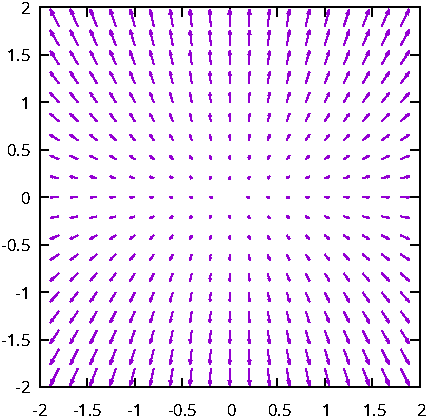
\includegraphics[width=.32\textwidth]{gnuplot/linear-pp-crop.pdf}
    \hfill
    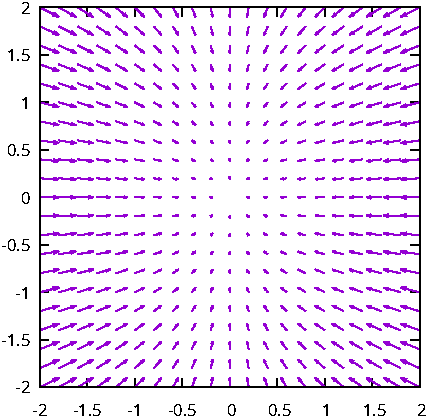
\includegraphics[width=.32\textwidth]{gnuplot/linear-mm-crop.pdf}
    \hfill
    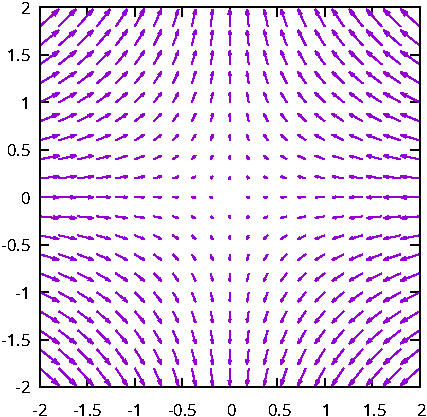
\includegraphics[width=.32\textwidth]{gnuplot/linear-pm-crop.pdf}
  \end{center}
\end{frame}

\begin{frame}
  \begin{exampleblock}{Diskussion}
    Reelle Matrizen können komplexe Eigenwerte haben. Offensichtlich
    wollen wir aber keine komplexwertigen Lösungen unserer AWA.
  \end{exampleblock}
\end{frame}

\begin{frame}{Komplexe Eigenwerte}
  \begin{block}{Satz}
    Hat eine reelle Matrix komplexe Eigenwerte, so treten sie als
    komplex konjugierte Paare mit ebensolchen Paaren von Eigenvektoren
    auf.
  \end{block}
  \pause
  Sei nun $r\pm i\phi$ ein solches Paar mit den Eigenvektoren $u\pm iv$
  \begin{align*}
    A (u\pm iv) &= {r+i\phi} (u\pm iv),\\
    e^A (u\pm iv) &= e^{r+i\phi} (u\pm iv) = e^r (\cos\phi \pm i \sin\phi)(u\pm iv).
  \end{align*}

  \vspace*{4cm}
\end{frame}

\begin{frame}
  \begin{block}{Reelle Lösungen}
    Hat die Matrix $A$ ein komplexes Eigenwertpaar
    $\lambda_{1/2} = r\pm i\phi$ mit zugehörigen Eigenvektoren
    $u\pm iv$, so ersetzen wir in der Transformationsmatrix die
    Eigenvektoren durch $u$ und $v$ und erhalten für $e^A$ eine
    quasi-Diagonalmatrix mit Block
    \begin{gather*}
      e^r
      \begin{pmatrix}
        \cos\phi & \sin\phi\\
        -\sin\phi & \cos \phi
      \end{pmatrix}
    \end{gather*}
  \end{block}
\end{frame}

\begin{frame}{Beispiele}
  \begin{center}
    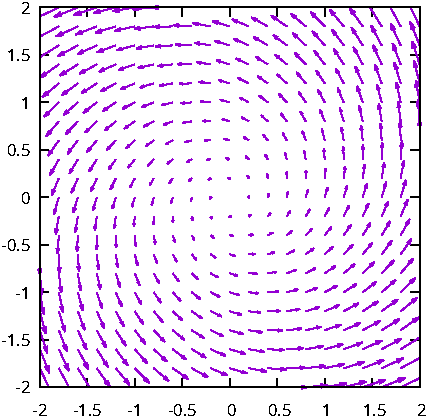
\includegraphics[width=.32\textwidth]{gnuplot/linear-cp-crop.pdf}
    \hfill
    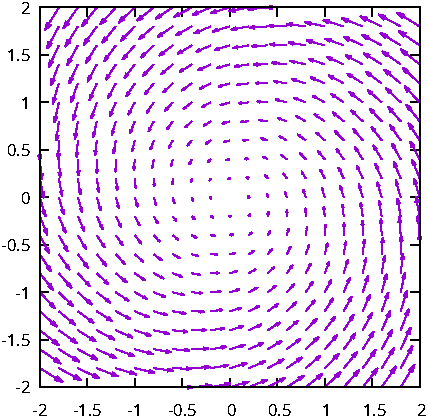
\includegraphics[width=.32\textwidth]{gnuplot/linear-cm-crop.pdf}
    \hfill
    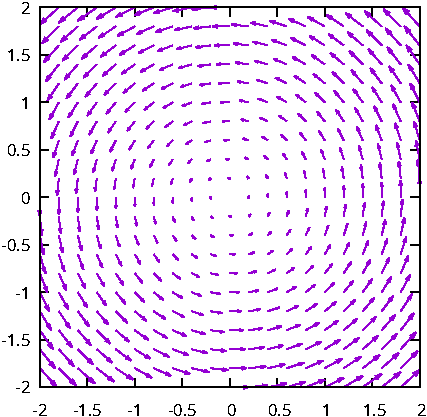
\includegraphics[width=.32\textwidth]{gnuplot/linear-c0-crop.pdf}
  \end{center}  
\end{frame}

%%%%%%%%%%%%%%%%%%%%%%%%%%%%%%%%%%%%%%%%%%%%%%%%%%%%%%%%%%%%%%%%%%%%%%
\subsection{Separable Gleichungen}
\frame{\subtoc}

\begin{frame}{Separation der Variablen}
  \begin{block}{Separable Gleichung}
    Eine DGl. der Form
    \begin{gather*}
      \frac{dx}{dt} = f(x)g(t)
    \end{gather*}
    heißt separabel.
  \end{block}

  \pause
  \begin{block}{Separationsansatz}
    \begin{enumerate}
    \item Schreibe die Gleichung in der Form
      \begin{gather*}
        \int \frac{dx}{f(x)} = \int g(t) \,dt.
      \end{gather*}
    \item Berechne beide Integrale
    \item Löse nach $x$ auf
    \end{enumerate}
  \end{block}
\end{frame}

\begin{frame}{Beispiel}
  \begin{gather*}
    x' = 2tx
  \end{gather*}
  \pause
  \begin{gather*}
    \int \frac1x\,dx = \int 2t \,dt
  \end{gather*}
  \pause
  \begin{gather*}
    \ln(x-c) = t^2
  \end{gather*}
  \pause
  \begin{gather*}
    x = e^{t^2}+c
  \end{gather*}
\end{frame}

%%%%%%%%%%%%%%%%%%%%%%%%%%%%%%%%%%%%%%%%%%%%%%%%%%%%%%%%%%%%%%%%%%%%%%
\subsection{Praktische Berechnung von Lösungen}
\frame{\subtoc}

\begin{frame}{Lösungen im Netz}
  Das Internet bietet uns viele Möglichkeiten zur Lösung von
  Differentialgleichungen
  \begin{itemize}
  \item Wikipedia
  \item Wolfram Alpha
  \item Suchfunktionen
  \item Generative KI
  \item Computeralgebrasysteme (CAS)
  \end{itemize}
\end{frame}

\begin{frame}{Kontrolle der Lösung}
  \begin{itemize}
  \item Das Lösen einer Differentialgleichung auf analytischem Wege mit
  \glqq{}Papier und Bleistift\grqq{} ist aufwändig und involviert
  schwierige Integrale.
\item Die Kontrolle, ob eine Lösung korrekt ist, erfordert nur das
  Gleichsetzen von Ableitungen. Dies ist einfach und stellt sicher,
  dass man selbst oder das Hilfsmittel korrekt gerechnet hat.
  \end{itemize}
\end{frame}

%%% Local Variables:
%%% mode: latex
%%% TeX-master: "slides.tex"
%%% End:
